\documentclass{beamer}

% importations de packages utiles
\usepackage[utf8]{inputenc}  % pouvoir écrire avec des accents
\usepackage[french]{babel}  % francophopnie
\usepackage{hyperref}  % liens clicables dans pdf final
\usepackage{tikz}  % pouvoir tracer des dessins sympas
\usetheme{Boadilla}  % thème de beamer
\usepackage{listingsutf8}  % rendu de "code" (avec config ci-dessous)
% configuration de lstlisting pour montrer du code python
\definecolor{lstcolor}{rgb}{0.9,0.95,0.95}
\definecolor{lstcommentcolor}{rgb}{0.,0.2,0.}
\lstset{
  frameround=tttt,
  %autogobble,
  frame=single,
  backgroundcolor=\color{lstcolor},
  % extendedchars=true,
  % basicstyle=\ttfamily\small,
  keywordstyle=\bfseries\color{blue},
  identifierstyle=\bfseries\color{red},
  stringstyle=\bfseries\color{orange},
  commentstyle=\color{lstcommentcolor},
  language=Python,
  keepspaces=True,
  basicstyle=\fontfamily{pcr}\selectfont\small, % monospace it for copypasting
  upquote=true,
  columns=flexible,
  showstringspaces=False,
  literate={é}{{\'e}}1
}

% table des matières locale
\newcommand\minitoc{
  \begin{frame}{\secname}
    \tableofcontents[currentsection, hideothersubsections, ] %  sectionstyle=show/show]
  \end{frame}
}
\newcommand\subminitoc{
  \begin{frame}{\secname}
    \tableofcontents[currentsubsection, hideothersubsections,
    sectionstyle=show/shaded, subsectionstyle=show/shaded, subsubsectionstyle=show]
  \end{frame}
}

% ignorer toute une section sans utiliser des % de commentaire
\newcommand\ignore[1]{}

% options pour la page de titre
\title{Projet \textit{RNG}}
\subtitle{Algorithmes et Structures de Données II}
\author{Juan-Carlos Barros, Yves Dethurens,\\ Daniel Kessler et Jean-Francis Ravoux}

% et c'est parti
\begin{document}
\begin{frame}
  \titlepage
\end{frame} % titre

\section{Introduction}
\minitoc
\subsection{À quoi servent les RNG?}
\begin{frame}{À quoi servent les Générateurs de Nombres Aléatoires?}
  \begin{center}
   
\includegraphics[width=.3\textwidth]{img/rng_dice.png}
   \includegraphics<2->[width=.4\textwidth]{img/rng_gaming.png}
  \par\medskip
  \includegraphics<3->[width=.8\textwidth]{img/dilbert_financial.png}
  \end{center}
  \end{frame}

\subsection{Que veut-on simuler?}
\begin{frame}{Que veut-on simuler?}
  \begin{itemize}
  \item Des $001101001\ldots$ aléatoires de la taille d'un \textbf{mot machine}\medskip
  \item<2-> Des nombres entre 0 et $2^{32} - 1$ ``tirés au hasard''
    \medskip
  \item<3-> Des nombres entre 0 et 1 \textbf{uniformément distribués}
  \end{itemize}
\end{frame}

\subsection{Vrai ou pseudo aléatoire?}
\begin{frame}
  \frametitle{Vrai ou pseudo aléatoire?}
  \begin{itemize}
  \item<1-> À partir de données ``physiques'' \onslide<3>{(TRNG)}
  \item<2-> Avec un algorithme déterministe  \onslide<3>{(PRNG)}
  \end{itemize}
  \begin{center}
    \begin{minipage}{0.33\textwidth}
    \includegraphics<1->[width=.7\textwidth]{img/xkcd_sports.png}
    \end{minipage}
    \begin{minipage}{0.65\textwidth}
    \includegraphics<2->[width=.8\textwidth]{img/xkcd_fair.png}
    \end{minipage}
    \par
    \onslide<2->{(source: xkcd.com)}
  \end{center}
\end{frame}

\section{Générateurs de nombres pseudo-aléatoires}
\minitoc
\subsection{Caractéristiques communes}
\begin{frame}
  \frametitle{Générateurs de nombres pseudo-aléatoires}
  Les Pseudo Random Number Generators (PRNG) génèrent:
  \begin{itemize}
  \item une \textbf{suite} de nombres de manière \textbf{déterministe} (et
    ``sans histoire'')
  \item<2-> à partir d'une \textbf{seed} (nombre initial)
  \item<3-> avec une certaine \textbf{période}\par
    (a priori limitée à $2^{32}$ pour des nombres à 32 bits, par exemple)
  \end{itemize}
\end{frame}

\subsection{Générateurs linéaires congruents (LCG)}
\begin{frame}{Générateurs linéaires congruents (LCG)}
  Pour l'instant ceci est un exemple de mise en page pour JF
  \begin{minipage}{0.32\textwidth}
    \onslide<1->{Du texte inutile gauche\par}
    \onslide<2->{Du texte inutile en plus}
  \end{minipage}
  \begin{minipage}{0.33\textwidth}
    Du texte inutile central
  \end{minipage}
  \begin{minipage}{0.32\textwidth}
    \only<1-2>{Du texte inutile droit}
    \only<3->{Un texte différent}
  \end{minipage}
\end{frame}

\subsection{Vrai chaos déterministe}
\subminitoc
\begin{frame}
\frametitle{Vrai chaos déterministe}
Le problème des générateurs basés sur la théorie des nombres, c’est qu’ils produisent des séquences périodiques, qui possèdent des propriétés qui rend la suite en partie prévisible, parce que les nombres générés sont dépendants de ceux qui les précédent. Ce qui ne se produit jamais dans une vraie suite aléatoire ! \\
D’autres générateurs, basés sur la théorie du chaos, sont imprévisibles (par définition, voir plus bas), mais il est généralement plus difficile de garantir que ceux-ci ont une période longue, et ils sont moins répandus que les générateurs basés sur la théorie des nombres. \\
Le générateur de nombres pseudo-aléatoires présenté ci-dessous (Saito \& Yamaguchi 2017) utilise les deux théories pour produire des suites qui ressemblent à de vraies suites aléatoires non périodiques. Son coût computationnel est élevé, mais les séquences générées peuvent par exemple servir de référence pour des tests qualitatifs. 
\end{frame}

\subsubsection{Décalage de Bernouilli}
\begin{frame}
\frametitle{Point de départ : décalage de Bernoulli}

La relation $\alpha_{n+1}=(2\alpha_n)\ mod\ 1$  définit une suite où $\alpha_n \in [0;1[$. En arrondissant les termes de cette suite, on obtient une séquence binaire pseudo-aléatoire. \\
Exemple : $\alpha_0$ = 0.3 donne la suite \{ 0.3; \textbf{0.6}; 0.2; 0.4; 0.8; \textbf{0.6}; … \} \\
ou la séquence 01001100110011001... qui est périodique et donc très prévisible. \\
Mais si $\alpha_0$ est \textbf{irrationnel}, cette suite devient \textbf{non périodique}. Cela signifie qu’une infinitésimale variation de $\alpha_0$ provoquera un changement radical à un moment de la séquence. Cette forte sensibilité aux conditions initiales est une caractéristique des fonctions chaotiques : au bout d'un certain temps, un phénomène chaotique devient imprévisible.
Une loi déterministe va évidemment être prévisible si ses paramètres sont entièrement connus. Mais si les conditions initiales contiennent une part d’incertitude (par exemple une imprécision, même minime), alors un tel processus chaotique ne permet plus de prévision à long terme.
\end{frame}

\begin{frame}
\frametitle{décalage de Bernoulli : annexe}
Exemple comparé, avec  $\alpha_0 = \frac{\pi}{4}$   et   $\overline{\alpha}_0 = \frac{355}{452}$, deux valeurs très proches :
\begin{tabular}{|*{7}{c|}}
\
& \multicolumn{3}{|c|}{suite irrationnelle} 
& \multicolumn{3}{|c|}{suite rationnelle} \\
$n$ & $\alpha_n$ & valeur & $\epsilon_n$ & $\overline{\epsilon}_n$ & valeur & $\overline{\alpha}_n$ \\ 
\hline
0 & $\pi/4$ & \textbf{0.78539816} & 1 & 1 & \textbf{0.78539823} & $\frac{355}{452}$ \\
1 & $\pi/2-1$ & 0.57079632 & 1 & 1 & 0.57079646 & $\frac{258}{452}$ \\
2 & $\pi-3$ & 0.14159265 & 0 & 0 & 0.14159292 & $\frac{64}{452}$ \\
3 & $2\pi-6$ & 0.28318530 & 0 & 0 & 0.28318584 & $\frac{128}{452}$ \\
4 & 4$\pi$‒12 & 0.56637061 & 1 & 1 & 0.56637168 & $\frac{256}{452}$ \\
5 & 8$\pi$‒25 & 0.13274122 & 0 & 0 & 0.13274336 & $\frac{60}{452}$ \\
6 & 16$\pi$‒50 & 0.26548245 & 0 & 0 & 0.26548672 & $\frac{120}{452}$ \\
7 & 32$\pi$‒100 & 0.53096491 & 1 & 1 & 0.53097345 & $\frac{240}{452}$ \\
8 & 64$\pi$‒201 & 0.06192982 & 0 & 0 & 0.06194690 & $\frac{28}{452}$ \\
9 & 128$\pi$‒402 & 0.12385965 & 0 & 0 & 0.12389380 & $\frac{56}{452}$ \\
10 & 256$\pi$‒804 & 0.24771931 & 0 & 0 & 0.24778761 & $\frac{112}{452}$ \\
11 & 512$\pi$‒1608 & 0.49543863 & 0 & 0 & 0.49557522 & $\frac{224}{452}$ \\
12 & 1024$\pi$‒3216 & 0.99087727 & 1 & 1 & 0.99115044 & $\frac{448}{452}$ \\
13 & 2048$\pi$‒6433 & 0.98175455 & 1 & 1 & 0.98230088 & $\frac{444}{452}$ \\
14 & 4096$\pi$‒12867 & 0.96350910 & 1 & 1 & 0.96460176 & $\frac{436}{452}$ \\
15 & 8192$\pi$‒25735 & 0.92701820 & 1 & 1 & 0.92920353 & $\frac{420}{452}$ \\
16 & 16384$\pi$‒51471 & 0.85403641 & 1 & 1 & 0.85840707 & $\frac{388}{452}$ \\
17 & 32768$\pi$‒102943 & 0.70807283 & 1 & 1 & 0.71681415 & $\frac{324}{452}$ \\
18 & 65536$\pi$‒205887 & 0.41614566 & 0 & 0 & 0.43362831 & $\frac{196}{452}$ \\
19 & 131072$\pi$‒411774 & 0.83229132 & 1 & 1 & 0.86725663 & $\frac{392}{452}$ \\
20 & 262144$\pi$‒823549 & 0.66458264 & 1 & 1 & 0.73451327 & $\frac{332}{452}$ \\
21 & 524288$\pi$‒1647099 & 0.32916528 & 0 & 0 & 0.46902654 & $\frac{212}{452}$ \\
22 & 1048576$\pi$‒3294198 & 0.65833057 & 1 & 1 & 0.93805309 & $\frac{424}{452}$ \\
23 & 2097152$\pi$‒6588397 & 0.31666114 & 0 & 1 & 0.87610619 & $\frac{396}{452}$ \\
23 & 4194304$\pi$‒13176794 & 0.63332228 & 1 & 1 & 0.75221238 & $\frac{340}{452}$ \\
24 & 8388608$\pi$‒26353589 & 0.26664456 & 0 & 1 & 0.50442477 & $\frac{228}{452}$ \\
25 & 16777216$\pi$‒52707178 & 0.53328913 & 1 & 0 & 0.00884955 & $\frac{4}{452}$ \\
26 & 33554432$\pi$‒105414357 & 0.06657826 & 0 & 0 & 0.01769911 & $\frac{8}{452}$ \\
27 & 67108864$\pi$‒210828714 & 0.13315653 & 0 & 0 & 0.03539823 & $\frac{16}{452}$ \\
28 & 134217728$\pi$‒421657428 & 0.26631307 & 0 & 0 & 0.07079646 & $\frac{32}{452}$ \\
29 & 268435456$\pi$‒843314856 & 0.53262615 & 1 & 0 & 0.14159292 & $\frac{64}{452}$ \\
\end{tabular}
\end{frame}

\subsubsection{Sensibilité aux conditions initiales}
\begin{frame}
\frametitle{décalage de Bernoulli : sensibilité aux conditions initiales}
On voit (cf.annexe) que les deux suites, malgré un point de départ presque identique, divergent complètement à partir de n = 20. Cela montre le caractère chaotique de la structure : sans la connaissance de la huitième décimale de $\alpha_0$,  impossible de prévoir le comportement de cette suite au-delà du 20e terme.\\
On sait dès lors que l’observation des 20 premiers termes ne permet pas d’en déduire la suite.\\  
\ \\
\textbf{Problème} : si on s’intéresse à la suite irrationnelle, parfaitement aléatoire en apparence, le problème est qu’il faut connaître le nombre irrationnel de départ (ici $\alpha_0 = \frac{\pi}{4}$) avec une précision croissante. Cela demandera un temps de calcul de plus en plus important, et ne ne sera plus possible pour de très grandes valeurs de $n$. \\
Il faut pouvoir gérer des valeurs exactes pour $\alpha_n$!
\end{frame}

\subsubsection{Racines irrationnelles du 3è degré}
\begin{frame}
\frametitle{Racines irrationnelles du 3e degré}
Saito et Yamaguchi (2017) proposent une solution à ce problème: en choisissant $\alpha_0$  comme racine d’un polynôme du 3e degré $f_0$ dont les coefficients sont entiers, et qui a une unique racine réelle. \\
Ainsi, on peut facilement déterminer le polynôme $f_1$ dont $\alpha_1$ est la racine, et ainsi de suite. \\
Exemple : on pose $f_0(x) = x^3+x–1$ et $f_n(x) = x^3+b_nx^2+c_nx–d_n$, avec $f_n(\alpha_n) = 0$, et $\epsilon_n = (\alpha_n)$.
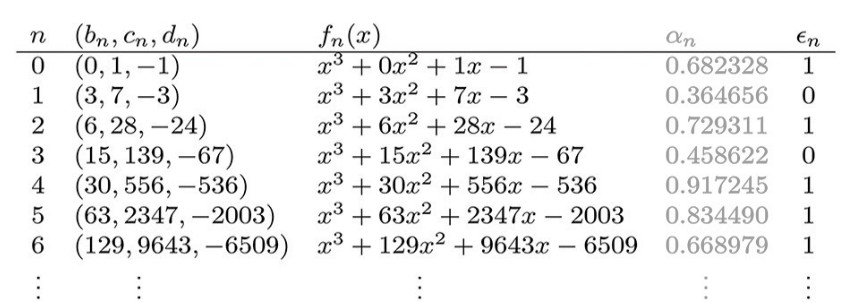
\includegraphics[scale=0.75]{img/SaitoYamaguchi2017.png}
\end{frame}

\subsubsection{Calcul de la séquence}
\begin{frame}
\frametitle{Calcul de la séquence}
Alors les relations ci-dessous permettent d'éviter le calcul des $\alpha_n$ : \\
\begin{tabular}{ l l }
$a_n$ = 1 & $b_{n+1}$ = $2b_n+3\epsilon_n$ \\ 
$c_{n+1} = 4c_n+(4b_n+3)\epsilon_n$ 
& $d_{n+1} = 8d_n+(4c_n+2b_n+1)\epsilon_n$ \\
\multicolumn{2}{l}{$1 + 2b_n + 4c_n + 8d_n < 0 \ \Leftrightarrow \ \alpha_n > \frac{1}{2} \ \Leftrightarrow \ \epsilon_n = 1 $}
\end{tabular} \\
\ \\
La production de la séquence pseudo-aléatoire $\{\epsilon_n\}_{n \in \mathbb{N}}$ consiste donc à déterminer les termes de la suite $\{ (b_n,c_n,d_n,\epsilon_n) \}_{n \in \mathbb{N}}$. Celle-ci se construit entièrement  avec des opérations élémentaires, sans avoir à extraire les racines $\alpha_n$ qui restent implicites. \\
\ \\
Selon les auteurs, en choisissant bien les coefficients du polynôme initial $f_0$, on peut vérifier que la séquence binaire produite est presque uniformément distribuée sur l’intervalle [0;1]. \\
\ \\
\textbf{Référence} : \\
\textit{Pseudorandom number generator based on the Bernoulli map on cubic algebraic integers}, 
Asaki Saito \& Akihiro Yamaguchi, 2017. 
\end{frame}

\section{Générateurs de nombres ``vraiment'' aléatoires}
\minitoc
\begin{frame}
  \frametitle{Générateurs de nombres ``vraiment'' aléatoires}
  Les True Random Number Generators (TRNG)\ldots\par
  \ldots à remplir par JC\ldots
\end{frame}
\subsection{Généralités - Processeur incapable}
\begin{frame}{Généralités - Processeur incapable}
\begin{itemize}
 \item Processeur arrive plutôt bien à propager de l’aléatoire
 \item Voir algorithmes présentés précédemment
 \item Mais il lui faut un coup de pouce au départ
 \item  Besoin d’une graine pour démarrer
 \item Pourquoi hasard inaccessible au processeur?
 \item Car le processeur est profondément déterministe
 \end{itemize}  
\end{frame}

\subsection{Généralités - Le Monde réel oui}
\begin{frame}{Généralités - Le Monde réel oui}
 \begin{itemize}
 \item Aléatoire inévitable et dérangeant dans le monde réel!
   \begin{itemize}
   \item Incertitudes fondamentales des mesures
   \item Impossibilité de contrôler une valeur physique
   \end{itemize}
 \item Monde réel est donc LA source d’inspiration
 \end{itemize}
\end{frame}

\subsection{Collection d'entropie}
\begin{frame}{Collection d'entropie}
  \begin{itemize}
  \item Principales sources de hasard:
    \begin{itemize}
    \item phénomènes physiques stochastiques:
      \begin{itemize}
      \item bruit thermique (Johnson et Nyquist)
      \item autres phénomènes statistiques (vagues, etc.)
      \end{itemize}
    \item phénomènes quantiques intrinsèquement aléatoires
      \begin{itemize}
      \item effet photoélectrique
      \item n’importe quelle autre mesure quantique
      \end{itemize}
    \end{itemize}
  \end{itemize}
\end{frame}

\subsection{Algorithmes d'aggrégation et expansion d'entropie}
\begin{frame}{Algorithmes d'aggrégation et expansion d'entropie}
 \begin{itemize}
 \item Algorithme pour grossir le flux de TRNG (pas assez rapide)
 \item HAVEGE (utilisé par le noyau Linux)
 \item HArdware Volatile Entropy Gathering and Expansion
 \item https://www.irisa.fr/caps/projects/hipsor/misc.php
 \end{itemize}
\end{frame}

\subsection{Le futur est-il quantique?}
\begin{frame}{Le futur est-il quantique?}
 \begin{itemize}
 \item Sources quantiques:
   \begin{itemize}
   \item source de radioactivité détectée par un compteur Geiger
   \item photons traversant un miroir semi-réfléchissant
   \item C’est le choix de la compagnie Genevoise ID Quantique
   \end{itemize}
 \end{itemize}
\end{frame}

\subsection{Exemple genevois: ID Quantique}
\begin{frame}{Exemple genevois: ID Quantique}
  \begin{itemize}
  \item Principe de la source ID Quantique:
    \begin{itemize}
    \item photons traversant un miroir semi-réfléchissant
    \item événements mutuellement exclusifs (réflexion / transmission)
    \item Détection associée respectivement à des valeurs de bit 0 ou 1
    \end{itemize}
  \end{itemize}
\end{frame}

\section{Que fait le module ``random'' de Python?}
\minitoc
\begin{frame}
  \frametitle{Que fait le module ``random'' de Python?}
  \begin{itemize}
  \item Python fait appel à l'OS pour le TRNG.\par
    \onslide<2->{L'OS implémente typiquement un algorithme HAVEGE.}
    \medskip
    \begin{itemize}
    \item<3-> utilisé directement par \texttt{random.SystemRandom} ou par
      \texttt{secrets}
      \par ce niveau d'aléatoire est nécessaire pour la cryptographie!
      \medskip
    \item<4-> utilisé en tant que \textit{seed} par défaut pour le PRNG de \texttt{random}
    \end{itemize}
    \bigskip
  \item<5-> Python utilise le \textbf{Mersenne Twister} en tant PRNG
    \begin{itemize}
    \item<6-> L'algorithme est plus complexe que ceux que nous avons présentés
      \medskip
    \item<7-> Il gère 624 nombres en parallèle, ce qui permet une période de
      $2^{19937}-1$, nettement plus que la limite naturelle de $2^{32}$.
    \end{itemize}
  \end{itemize}
\end{frame}
\begin{frame}[containsverbatim]{Que fait le module ``random'' de Python?}
  Le module \texttt{random} fournit des fonctions transformant directement ces
  nombres pour émuler des distributions aléatoires usuelles, le tirage sans
  remise, etc.
  \bigskip
  
\begin{lstlisting}
import random

# entier aléatoire entre 0 et 9
n = random.randrange(10)

# flottant aléatoire entre 0 et 10
x = random.uniform(0, 10)

# tirage de 2 éléments au hasard d'une liste
l = random.sample(["a", "b", "c", "d", "e"], 2)
\end{lstlisting}
\end{frame}

\ignore{ % par le temps, on devra zapper - mais on garde le code ici si jamais
\begin{frame}
  \frametitle{Distributions aléatoires discrètes}
  \begin{itemize}
  \item $f(x)$, la ``fréquence'' de $x$, est la probabilité de tirer $x$.
  \item $f(x)\geq0, \;\forall x$
  \item $\sum_xf(x)=1$
  \end{itemize}
  \begin{tabular}{ccc}
    \onslide<2->{
    \begin{tikzpicture}[scale=.5, every node/.style={scale=0.5}]
      \draw[->] (-.2,0) -- (5.5,0) node[right] {$x$};
      \draw[->] (0, -0.2) -- (0, 4.2) node[above] {$f(x)$};
      \foreach \i in {1, ..., 5} {
        \draw[blue] (\i, 0) -- (\i, 3.5);
        \node at (\i, -0.3) {$\i$};
      }
      \draw (.1, 3.5) -- (-.1, 3.5) node[left] {$0.2$};
    \end{tikzpicture}}
    &\onslide<3->{
      \begin{tikzpicture}[scale=.5, every node/.style={scale=0.5}]
        \draw[->] (-1.2,0) -- (5.2,0) node[right] {$x$};
        \draw[->] (-1,-0.2) -- (-1,6.2) node[above] {$f(x)$};
        \draw[blue] (0, 0) -- (0, 1);
        \draw[blue] (1, 0) -- (1, 4);
        \draw[blue] (2, 0) -- (2, 6);
        \draw[blue] (3, 0) -- (3, 4);
        \draw[blue] (4, 0) -- (4, 1);
        \foreach \i in {0, ..., 5} {
          \node[below] at (\i, 0) {$\i$};
        }
      \end{tikzpicture}}
    &\onslide<4->{
      \begin{tikzpicture}[scale=.5, every node/.style={scale=0.5}]
        \draw[->] (-1.2,0) -- (4.2,0) node[right] {$x$};
        \draw[->] (-1,-0.2) -- (-1,4.2) node[above] {$f(x)$};
        \node[blue] at (1.5, 2) {\Huge ?};
      \end{tikzpicture}}
    \\
    \onslide<2->{uniforme} & \onslide<3->{binômiale} & \onslide<4->{autre}
  \end{tabular}    
\end{frame}
\begin{frame}
  \frametitle{Distributions aléatoires continues}
  \begin{itemize}
  \item $\int_a^bf(x)$ est la probabilité de tirer $x$ entre $a$ et $b$.
  %\item $f(x)\geq0, \;\forall x$
  \item $\int_{-\infty}^{+\infty}f(x)=1$
  \end{itemize}
  \begin{tikzpicture}
    \draw[->] (-.2,0) -- (4.2,0) node[right] {$x$};
    \draw[->] (0,-0.2) -- (0,2.2) node[above] {$f(x)$};
    \draw[blue] (1, 0) -- (1, 1) -- (3, 1) -- (3, 0);
    \draw (1, .1) -- (1, -.1) node[below] {\small$c$};
    \draw (3, .1) -- (3, -.1) node[below] {\small$d$};
    \node at (2, 2.2) {uniforme};
    \onslide<2->{
    \def\dx{6.8}; \def\dy{-3};
    \draw[->] (-4.2+\dx, \dy) -- (4.2+\dx,\dy) node[right] {$x$};
    \draw[->] (\dx-1,\dy-.2) -- (\dx-1, 2.2+\dy) node[above] {$f(x)$};
    \draw[blue] (\dx, \dy) plot[domain=-4:4, samples=200] ({\x+\dx},{\dy+2*2^(-\x*\x)});
    \draw (\dx, .1+\dy) -- (\dx, \dy-.1) node[below] {\small$\mu$};
    \def\ec{1.3}
    \draw (\dx+\ec, .1+\dy) -- (\dx+\ec, \dy-.1) node[below] {\small$\mu+\sigma$};
    \draw (\dx-\ec, .1+\dy) -- (\dx-\ec, \dy-.1) node[below] {\small$\mu-\sigma$};
    \node at (\dx+1, \dy+2.3) {normale};
    }\onslide<3->{
    \def\dx{8}; \def\dy{.5};
    \draw[->] (\dx-.2, \dy) -- (\dx+3.2,\dy) node[right] {$x$};
    \draw[->] (\dx-.1,\dy-.2) -- (\dx-.1, \dy+2.2) node[above] {$f(x)$};
    \node[blue] at (\dx+1.5, \dy+1) {\Huge ?};
    \node at (\dx+1.5, \dy+2.2) {autre};
    }
  \end{tikzpicture}
\end{frame}
}
\end{document}
